\documentclass[conference]{IEEEtran}
\IEEEoverridecommandlockouts
% The preceding line is only needed to identify funding in the first footnote. If that is unneeded, please comment it out.
%\usepackage{cite}
\usepackage{amsmath,amssymb,amsfonts}
\usepackage{algorithmic}
\usepackage{graphicx}
\usepackage{textcomp}
\usepackage[table,xcdraw]{xcolor}
\usepackage{paralist} % compactitem etc
\usepackage{booktabs} % For formal tables
\usepackage{numprint}
\usepackage{xspace}
%\usepackage{cite}
\usepackage{amsmath,amssymb,amsfonts}
\usepackage{color}
\usepackage{textcomp}
\usepackage[normalem]{ulem}
\usepackage{soul}
\usepackage{multirow}
\usepackage{multicol}
\usepackage{footmisc}
\usepackage{dblfloatfix}
\usepackage{listings}
\usepackage[utf8]{inputenc}
\usepackage[english]{babel}
\usepackage[noadjust]{cite}
\usepackage{listings}
\usepackage{minted}
\usepackage{amsthm}
\usepackage{amssymb}
\usepackage{pdfrender}

% If you use beamer only pass "xcolor=table" option, i.e. \documentclass[xcolor=table]{beamer}
\usepackage[normalem]{ulem}
\useunder{\uline}{\ul}{}

\usepackage[table,xcdraw]{xcolor}
%\usepackage[noline,noend]{algorithm2e}
\usepackage[noline]{algorithm2e}
\usepackage{url}
\def\UrlFont{\rmfamily}

\usepackage[colorinlistoftodos]{todonotes}
\newcommand{\ignore}[1]{ } % ignore blocks of text
\newcommand{\maketiny}[1]{{\tiny G: #1}} % ignore blocks of text
\newcommand{\ganesh}[1]{\todo[inline,size=\small, color=purple!40]{G: #1}}



\newcommand{\goat}{\textsc{GoAT}\xspace}

\newcommand{\etc}{etc.\@\xspace}
\newcommand{\ie}{i.e.\@\xspace}
\newcommand{\eg}{e.g.\@\xspace}

%% colors
\newcommand{\tbl}[1]{\textcolor{blue}{#1}}
\newcommand{\tb}[1]{\textcolor{black}{#1}}
\newcommand{\tr}[1]{\textcolor{red}{#1}}
\newcommand{\tg}[1]{\textcolor{green}{#1}}

\newcommand\ggcmt[1]{\todo[inline, size=\small, color=green!40]{GG: #1}}
\newcommand\ggcmtside[1]{\todo[size=\scriptsize, color=green!40]{GG: #1}}

\newcommand\stcmt[1]{\todo[inline, size=\small, color=orange!60]{#1}}
\newcommand\stcmtside[1]{\todo[size=\scriptsize, color=orange!40]{#1}}

%--\newcommand{\circleRtool}{circleRtool\circledR\xspace}

%%% Local Variables:
%%% mode: latex
%%% eval: (flyspell-mode 1)
%%% TeX-master: "root.tex"
%%% End:


\renewcommand{\algorithmcfname}{Procedure}




\newtheorem{definition}{Definition}[section]

\makeatletter
\def\BState{\State\hskip-\ALG@thistlm}
\makeatother

\definecolor{codegreen}{rgb}{0,0.3,0}
\definecolor{codegray}{rgb}{0.5,0.5,0.5}
\definecolor{codepurple}{rgb}{0.58,0,0.82}
\definecolor{backcolour}{rgb}{0.98,0.98,0.98}

\lstdefinestyle{mystyle}{
    backgroundcolor=\color{backcolour},
    commentstyle=\color{codegreen},
    keywordstyle=\color{magenta},
    numberstyle=\tiny\color{codegray},
    stringstyle=\color{codepurple},
    basicstyle=\ttfamily\scriptsize,,
    breakatwhitespace=false,
    breaklines=true,
    captionpos=b,
    keepspaces=true,
    numbers=left,
    numbersep=4pt,
    showspaces=false,
    showstringspaces=false,
    showtabs=false,
    tabsize=2,
    morekeywords={pragma, omp}
}

\lstset{style=mystyle}
\lstset{escapeinside={<@}{@>}}



\def\BibTeX{{\rm B\kern-.05em{\sc i\kern-.025em b}\kern-.08em
    T\kern-.1667em\lower.7ex\hbox{E}\kern-.125emX}}
\begin{document}


\title{\goat: Automated Concurrency Analysis and Debugging Tool for Go}


%\author{\IEEEauthorblockN{Saeed Taheri}
%\IEEEauthorblockA{\textit{School of Computing} \\
%\textit{University of Utah}\\
%Salt Lake City, U.S.A. \\
%staheri@cs.utah.edu}
%\and
%\IEEEauthorblockN{Ganesh Gopalakrishnan}
%\IEEEauthorblockA{\textit{School of Computing} \\
%\textit{University of Utah}\\
%Salt Lake City, U.S.A. \\
%ganesh@cs.utah.edu}
%}

\maketitle

\begin{abstract}
%%% -*-LaTeX-*-
%%% This is the abstract for the thesis.
%%% It is included in the top-level LaTeX file with
%%%
%%%    \preface    {abstract} {Abstract}
%%%
%%% The first argument is the basename of this file, and the
%%% second is the title for this page, which is thus not
%%% included here.
%%%
%%% The text of this file should be about 350 words or less.

With the high growth in computation power and the invention of modern languages, concurrent software testing and debugging is vital to deliver reliable software.
%
Finding bugs in concurrent/parallel software is notoriously challenging because 1) the interleaving space grows exponentially with the number of processing units (\eg, CPU cores), 2) the nondeterministic nature of concurrent software makes concurrent bugs difficult to reproduce, and 3) root-causing misbehaved executions of a concurrent program is nontrivial due to the complex interactions between concurrent components of the program.
%
In this work, we have designed and implemented several frameworks and toolchains to overcome large-scale and real-world concurrent/parallel software debugging challenges.
%
Our methods aim to facilitate the concurrent debugging process by providing efficient data collection and effective information retrieval mechanisms to target real-world software and bugs.
%
First, we introduce \parlot, a whole-program call tracing framework for HPC applications (MPI+X) that highly compresses the traces (up to more than 21000 times) while adding minimal overhead with an average required bandwidth of just 56 kB/s per core.
%
Second, we present DiffTrace, a series of automated data abstraction, representation, and visualization techniques that differentiate the collected \parlot traces and narrows the search space down to just a few candidates of buggy traces.
%
Finally, we illustrate \goat, an end-to-end framework for automated tracing, analysis, and testing of concurrent Go applications.
%
We also propose a set of coverage metrics to measure the quality of schedule exploration in CSP-like concurrent languages.
%
Our evaluation of \goat on a recent Go concurrency bug benchmark of real-world programs shows a 100\% success rate in detecting blocking bugs.

\end{abstract}

\begin{IEEEkeywords}
golang, concurrency, testing coverage analysis
\end{IEEEkeywords}

\bstctlcite{IEEEexample:BSTcontrol}

%\section{GIntroduction}
%\label{sec:Gintro}
%
The use of increasing levels of parallelism and concurrency in HPC and Cloud
is a double-edged sword: while it helps increase performance, save energy, and
enhance user experience, it
unfortunately comes with the cost of concurrency bugs.
%
This trend can worsen with the upcoming HPC/Cloud
integration~\cite{dan-herbein-dong} unless we accelerate the
development of concurrency debugging methods.
%
However, unless these debugging systems themselves are
simple and widely applicable,
the maintenance of multiple debugging approaches
will also prove to be a burden.
%
Driven by these observations,
in this paper we take a feature-rich language, namely Go~\cite{go-citation},
research how to develop an effective debugging methods for real-world
Go programs, and present the resulting new tool called GoAT.
%
The main contribution of this work is to demonstrate how
GoAT's static and dynamic analysis methods---while very well known
by their names and effectiveness in simpler contexts---can
be brought to bear on realistic bug-scenarios in the setting of
a complex language such as Go; this is our central contribution.


Go enjoys accelerating acceptance in a wide variety of
communities---especially the Cloud community.
%
It involves shared memory, message passing, nondeterministic
message reception and selection,
dynamic process creation,
and programming styles that tend to create thousands of Go routines
and discard them to be garbage collected when not needed.
%
This combination of features is known to be the reason why Go
is popular; yet, it is also well recognized that these features also make
Go debugging hard.
%
Our work is especially relevant considering that
there are there no widely usable tools for debugging Go; even well-curated
bug benchmark suites are only just
now beginning to appear~\cite{tu-concurrentBugs-asplos19,yuan-gobench-cgo21}.
%
Combinations of Go's features are found in many other languages,
making our study carry a broader degree of relevance
to the HPC/Cloud ecosystem, in addition to providing an effective
tool for Go itself.


One of our priorities in designing GoAT
was to reuse as much of the existing Go infrastructure
as we could.
%
The static analysis component relies on source rewriting, inserting
{\em potential} schedule yield points
at all
``interesting'' (concurrency-relevant) spots inside a given Go program.
%
The dynamic component consists of yielding control back
to the Go runtime with a user-settable probability value.
%
Last but not least, we also exploited the tracing features of Go
to provide, via GoAT, (1)~as much debug information as possible, and
(2)~use the tracing features to measure and report concurrency coverage.


Our preliminary results in terms of this combined static/dynamic
approach yielded encouraging results.
%
However, bug-hunting on curated bug data sets cannot, by itself, give any
indications on how well an approach might {\em generalize}.
%
Generalization in terms of debugging tools is often achieved
by carefully defining {\em coverage metrics} and showing how
well these metrics are met.
%
Again, we walked into a field with very few such coverage metrics.


Our coverage metrics
are clearly inspired by other concurrrency coverage
metrics~\cite{cite,a,few,of,them}.
%
Overall, our coverage metrics are inspired by real-world Go bugs,
and this is new in terms of debugging Go concurrrency.
%
Also coverage metrics for select statements---high in the list of
Go bugs---are believed to be novel.
%
Last but not least, we also differentiate between covering
easier bugs and rare bugs: the former do not require any
schedule control, while the latter is triggered only through schedule
control.


Developing these coverage metrics required studying the output
of our initial
tracing infrastructure on Go bug benchmarks.
%
We take advantage of our own tracing framework to
tabulate and report on the achieved coverage metrics.
%
All this is offered via a new tool called \goat (Go Analysis and Testing Tool)
that we now describe, after introducing relevant features of Go
itself.


\noindent{\bf Features of Go:\/}
Go \cite{go} is a statically typed language initially developed by Google and at present widely used by many.
%
It employs channel-based Hoare's Communicating Sequential Processes (CSP) \cite{hoare-csp78} semantics in its core and provides a productivity-enhancing environment for concurrent programming.
%
The concurrent model in Go centers around
1) \textit{goroutines} as light-weight user-level threads (processing units),
2) \textit{channels} for explicit messaging to synchronize and share memory through communication, and
3) a \textit{scheduler} that orchestrates goroutine interactions while shielding
the user from
many low-level
aspects of the runtime.
%
This design
facilitates the
construction
of data flow models that efficiently utilize multiple CPU cores.
%
Because of the simple yet powerful concurrency model, many real production software systems take advantage of Go,
including
container software systems such as Docker \cite{merkel2014docker}, Kubernetes \cite{kubernetes},  key-value databases \cite{etcd}, and web server libraries \cite{grpc}.
%


In traditional shared-memory concurrent languages such as Java/C/C++, threads interact with each other via shared memory.
%
Processes in CSP-based languages such as Erlang communicate through mailbox (asynchronous) message passing.
%
Go brings all these features together into one language and encourages developers to \textit{share memory through communication} for safe and straightforward concurrency and parallelism.
%
The visibility guarantee of memory writes is specified in the memory model\cite{go-memModel} under synchronization constraints (\textit{happens-before} partial order \cite{lamport-hb-1978}).
%
The language is equipped with a rich vocabulary of \textit{serialization} features to facilitate the memory model constraints; they include synchronous and asynchronous communication (either unbuffered or buffered channels), memory protection, and barriers for efficient synchronization.
%
This rich mixture of features has, unfortunately, greatly exacerbated the complexity of Go debugging.
%
In fact, the popularity of Go has outpaced its debugging support~\cite{go-survey,tu-concurrentBugs-asplos19,dilley-empirical-saner19}.
%
There are some encouraging developments in support of debugging, such as a data race checker \cite{go-race-blog} that has now become a standard feature of Go, and has helped catch many a bug.
%
However, the support for ``traditional concurrency debugging'' such as detecting atomicity violations and Go-specific bug-hunting support for Go idioms (e.g., misuse of channels and locks) remain insufficiently addressed.
%

\noindent{\bf Contributions:\/} In
this work, we present the initial steps that we took towards addressing this lack.
%
Since a bug might
occur
at various levels of abstraction, dynamic tracing provides a practical and uniform way to track multiple facets of the program during execution (as we have shown in our prior work~\cite{difftrace}).
%
Also, unlike assertion-based tools \cite{lange-staticType-icse18,wolf-gobra-cav21}, a dynamic tool is more automated, not requiring user expertise.
%
We developed a facility that automatically gathers \textit{execution concurrency traces} (\ie sequences of events) during the execution of Go applications with minimal instrumentation.
%
By enhancing the Go built-in tracing mechanism with \textit{concurrency usage} events, we enrich original \textit{execution traces} so that they accurately reflect the dynamic concurrency behavior of applications.
%
Upon Go programs' termination when tracing is enabled, traces are flushed and structurally stored in relational tables of an SQL database, enabling multi-aspect program analysis in offline.
%

With the help of this novel \textit{automated dynamic tracing} mechanism,
we have implemented a testing framework that
\textit{accelerates} bug exposure by manipulating the native scheduler around \textit{critical points} in the code---combination of constructs that heighten the propensity for bug-introduction.
%



To summarize, here are our contributions:
\stcmtside{need to update}
\begin{itemize}
    \item We take the tracing mechanism embedded in the standard Go that captures \textit{execution trace} (ET) and enhance it with a set of concurrency primitive usage events to obtain \textit{execution concurrency trace} (ECT). While the primary usage of ET is performance analysis, ECT provides an accurate and comprehensive model of concurrent execution, enabling automated analysis of logical behavior and concurrent bug detection.
    \item We introduce a framework that automatically instruments the target program, collects ECT, and structurally stores them in a database. Through querying the database, several visualizations and reports are accessible.
    \item We propose an approach to identify the points (\ie source line number) in the target program in which a random noise might drastically change the program's dynamic behavior. We analyze ECTs to identify such points and measure schedule space coverage per execution.
    \item Coverage metric
\end{itemize}
\stcmtside{need to update}
The rest of this paper is as follows: Section \ref{sec:correctness} discusses correctness problems and approaches in Go. Section \ref{sec:ect} describes the enhancement we made to the tracer package. Section \ref{sec:disc} discusses the advantages of dynamic tracing for concurrent debugging and draws the ongoing and future direction of the current work. At last, Section \ref{sec:summary} summarizes and concludes.


\section{Introduction}
\label{sec:intro}
Debugging high-performance computing code
remains a challenge at all levels of scale.
%
Conventional HPC debuggers~\cite{ddt,totalview}
excel at many tasks such as examining the execution
state of a complex simulation in detail
and allowing the developer to re-execute
the program close to the point of failure.
%
However, they do not provide a good understanding
of why a program version that worked earlier
failed upon upgrade or feature addition.
%
Innovative solutions are needed to highlight the
salient differences between two executions in a manner
that makes debugging easier as well as more systematic.
%
A recent study conducted under the auspices of the
DOE~\cite{hpcdoe}
provides a comprehensive survey
of existing debugging tools.
%
It classifies them under
four software organizations (serial, multithreaded,
multi-process, and hybrid), six
method types (formal methods, static analysis, dynamic
analysis, nondeterminism control, anomaly detection,
and parallel debugging), and lists a total of 30 specific
tools.
%
Despite this abundance of activity and tools, many
significant problems remain to be solved before debugging
{\em can be approached by the HPC community as a collaborative
activity} so that HPC developers can extend a common
framework.


Almost all debugging approaches seek to find outliers (``unexpected
executions'') amongst thousands of running processes and threads.
%
The approach taken by most existing tools is to
look for symptoms in a specific bug-class that they cover.
%
Unfortunately,
this approach calls for a programmer having a good guess of what
the underlying problem might be,
and to then pick the right set of tools to deploy.
%
If the guess is wrong, the programmer has no choice but to
refine their guess
and look for bugs in another class,
re-executing the application and hoping for
better luck with another tool.
%
This iterative loop of re-execution followed by applying a
best-guess tool for the suspected bug class can potentially consume
large amounts of execution cycles and wastes an
expert developer's time.
%
More glaring is the fact that these tools must recreate the
execution traces yet again: they do not have means to hand off
these traces to another tool or cooperate in symbiotic ways.



We cannot collect all relevant pieces of information
necessary to detect all possible bug classes such as
resource leaks, deadlocks, and data races.
%
Each such bug requires its attributes to be kept.
%
Also, debugging is not fully automatable (it is
an undecidable problem in general) and must involve human thinking:
at least to reconcile what is observed against the deeper application-level semantics.
%
However, (1)~we believe that it is still possible to collect one standard set
of data and use it to make an initial triage in such
a way that it can guide a later, deeper debugging phase to locate
which of the finer bug gradations (e.g., resource leaks or races) brought
the application down.
%
Also, (2)~we believe that it is possible to engage the human {\em with respect
to understanding structured presentations of information}.



Our DiffTrace framework addresses both issues.
%
The common set of data it uses is a {\em whole program
function call trace} collected per process/thread.
%
DiffTrace relies on
novel ways to diff a normal trace and a fault-laden trace to guide the
debugging engineer closer to the bug.
%
While our work has not (yet) addressed situations in
which millions of threads and thousands of processes run
for days before they produce an error,
we strongly believe that we can get there
once we understand the pros and cons of our initial
implementation of the DiffTrace tool, which is described in this paper.
%
The second issue is handled in DiffTrace by offering a novel
collection of modalities for understanding program execution diffs.
%
We now elaborate on these points by addressing the following three problems.



\subsection{Problem 1 -- Collecting Whole-Program Heterogeneous Function-Call Traces
Efficiently\/} Not only must we have the ability
to record function calls and returns at one
API such as MPI, increasingly we must collect calls/returns at multiple
interfaces (e.g., OpenMP, PThreads, and even inner levels such as TCP).
%
The growing use of heterogeneous parallelization necessitates that we
understand MPI and OpenMP activities (for example) to locate cross-API
bugs that are often missed by other tools.
%
Sometimes, these APIs contain the actual error (as opposed to the user code), and it would be attractive to have this debugging ability.


{\em Solution to Problem 1:\/}
In DiffTrace, we choose Pin-based whole program binary tracing, with
tracing filters that allow the designer to collect a suitable mixture of API
calls/returns.
%
We realize this facility using
ParLOT, a tool designed by us and published earlier~\cite{parlot}.
%
In our research, we have thus far demonstrated the advantage of
ParLOT with respect to collecting both MPI and OpenMP traces
from a {\em single run of a hybrid MPI/OpenMP program}.
%
We demonstrate that, from this single type of trace, it is possible
to pick out MPI-level bugs and/or OpenMP-level bugs.
%
While whole-program tracing
may sound extremely computation and storage intensive, ParLOT employs
lightweight on-the-fly compression techniques to keep these overheads low.
%
It achieves compression ratios exceeding 21,000~\cite{parlot},
thus making this approach practical, demanding
only a few kilobytes per second per core of bandwidth.


\subsection{Problem 2 -- Need to Generalize Techniques for Outlier Detection\/}
Given that outlier detection is central to debugging,
it is essential to use efficient representations of the traces
to be able to systematically compute
{\em distances} between them without
involving human reasoning.
%
The representation must also be versatile enough to
be able to ``diff'' the traces
with respect to {\em an extensible number of vantage points}.
%
These vantage points could be diffing traces concerning process-level activities,
thread-level activities, a combination thereof,
or even finite sequences of process/thread calls (say, to locate {\em changes}
in caller/callee relationships).


{\em Solution to Problem 2:\/}
DiffTrace employs {\em concept lattices} to amalgamate the collected traces.
%
Concept lattices have previously been employed in HPC to perform structural
clustering of process behaviors~\cite{weberStructural} to present performance data more
meaningfully to users.
%
The authors of that paper use the notion of {\em Jaccard distances}
to cluster performance results that are closely related to process structures
(determined based on caller/callee relationships).
%
In DiffTrace, we employ incremental algorithms for building and maintaining
concept lattices from the ParLOT-collected traces.
%
In addition to Jaccard distances, in our work, we also perform hierarchical
clustering of traces and provide a tunable threshold for outlier detection.
%
We believe that these uses of concept lattices and refinement approaches
for outlier detection are new in HPC debugging.


\subsection{Problem 3 -- Loop Summarization\/}
Most programs spend most of their time in loops.
%
Therefore, it is important to employ state-of-the-art algorithms for
loop extraction from execution traces.
%
It is also important
to be able to diff two executions with respect to changes in their looping behaviors.
%
In our experience, presenting such changes using good visual metaphors
tends to highlight many bug types immediately.


{\em Solution to Problem 3:\/}
DiffTrace utilizes the rigorous notion of Nested Loop Representations (NLRs) for
summarizing traces and representing loops.
%
Each repetitive loop structure is given an identifier, and nested loops are
expressed as repetitions of this identifier exponentiated (as with regular
expressions).
%
This approach to summarizing loops can help manifest
bugs where the program does not hang or crash but nevertheless
runs differently in a manner that informs the developer engaged in debugging.

{\bf Organization\/}:
%
\S\ref{sec:ch3_overview} illustrates the contributions of this paper on a simple example.
%
\S\ref{sec:ch3_algo} presents the algorithms underlying DiffTrace in more detail.
%
\S\ref{sec:ch3_ilcs-case-study} summaries the experimental methodology before showing a medium-sized case study involving MPI and OpenMP.
%
\S\ref{sec:ch3_lulesh} shows initial measurements and examples on LULESH~\cite{LULESH2:changes}, a DOE common mini app.
%
\S\ref{sec:ch3_related} summarizes selected related works.
%
\S\ref{sec:ch3_discussion} concludes the paper with a discussion.

%
% \Noindent To summarize, the key contributions of this paper are the following
% \begin{itemize}
% \item A method to organize function call traces collected from processes and
%       threads into concept lattices, and a method to
%       detect loops from dynamic traces (Section~\ref{sec3}).
%
% \item Details of the algorithms employed in DiffTrace (Section~\ref{sec4}).
%
% \item Experimental studies on a heterogeneous program called
%       Iterated Local Champion Search (ILCS, Section~\ref{sec5}).
%
% \item Strengths and limitations of DiffTrace, plans for future work (Section~\ref{sec6}).
% \end{itemize}
%



\section{Background}
\label{sec:bg}
Recording a log of events during the execution of an application is essential for better understanding the program behavior and, in case of a failure, to locate the problem.
%
Recording this type of information requires instrumentation of the program either at the source-code or the binary-code level.
%
Instrumenting the source code by adding extra libraries and statements to collect the desired information is easy for developers.
%
However, doing so modifies the code and requires recompilation, often involving multiple different tools and complex hierarchies of makefiles and libraries, which can make this approach cumbersome and frustrating for users.
%
Instrumenting an executable at the binary level using a tool is typically easier, faster, and less error prone for most users.
%
Moreover, binary instrumentation is language independent, portable to any system that has the appropriate instrumentation tool installed, and provides machine-level insight into the behavior of the application.
%

\subsection{Binary Instrumentation}
Executables can be instrumented \textit{statically}, where the additional code is inserted into the binary before execution, which results in a persistent modified executable, or \textit{dynamically}, where the modification of the executable is not permanent. In dynamic binary instrumentation, code behavior can be monitored at runtime, making it possible to handle dynamically-generated and self-modifying code. Furthermore, it may be feasible to attach the instrumentation to a running process, which is particularly useful for long-running applications and infinite loops.

Many different tools for investigating application behavior have been designed on top of such Dynamic Binary Instrumentation (DBI) frameworks. For instance, Dyninst~\cite{dyninst} provides a dynamic instrumentation API that gives developers the ability to measure various performance aspects. It is used in tools like Open-SpeedShop~\cite{openss} and TAU~\cite{tau} as well as correctness debuggers like STAT~\cite{stat}. Moreover, VampirTrace~\cite{vampirt} uses it to provide a library for collecting program execution logs. 

Valgrind~\cite{valgrind} is a shadow-value DBI framework that keeps a copy of every register and memory location. It provides developers with the ability to instrument system calls and instructions. Error detectors such as Memcheck~\cite{memcheck} and call-graph generators like \callgrind~\cite{callgrind} are built upon Valgrind.\footnote{Given the absence of tools similar to \parlot, we employ \callgrind
 as a ``close-enough'' tool in our comparisons elaborated in \S\ref{sec:tracing-tools}.
 In this capacity, \callgrind is similar to \parlotm, a variant of \parlot that only collects
 traces from the {\tt main} image. We perform such comparison to have an idea of how we fare
 with respect to one other tool. In \S\ref{sec:results}, we also present a self-assessment of \parlot separately.}

 
%


We implemented \parlot on top of \pin~\cite{pin}, a DBI framework for the IA-32, x86-64, and MIC instruction-set architectures for creating dynamic program analysis tools. There is also version of \pin available for the ARM architecture \cite{pinarm}. \parlot mutates \pin to trace the entry (call) and exit (return) of every executed function. Note that our tracing and compression approaches can equally be implemented on top of other instrumentation tools. For example, PMaC \cite{pmac} is a DBI tool for the PowerPC/AIX architecture upon which \parlot could also be based.


\subsection{Efficient Tracing}
When dealing with large-scale parallel programs, any attempt to capture reasonably frequent events will result in a vast amount of data. Moreover, transferring and storing the data will incur significant overhead. For example, collecting just one byte of information per executed instruction yields on the order of a gigabyte of data per second on a single high-end core. Storing the resulting multi-gigabyte traces from many cores can be a challenge, even on today's large hard disks.

Hence, to be able to capture whole-program call traces, we need a way to decrease the space and runtime overhead. \textit{Compression} can encode the generated data using a smaller number of bits, help
reduce the amount of data movement across the memory hierarchy, and
lower storage and network demands.
%
Although the encoded data will later have to be decoded for analysis, compressing them during tracing enables the collection of {\em whole-program} traces.

The use of compression by itself is not new.
Various performance evaluation tools~\cite{tau,scorep,eventflowgraph} 
already employ compression during the collection
of performance analysis data.
%
Tools such as ScalaTrace~\cite{scalatrace}
also exploit
the repetitive nature of time-step simulations~\cite{freitag}. Aguilar et al. \cite{aguilar} proposed a lossy compression mechanism using the Nami library \cite{gamblinNami} for online MPI tracing. Mohror and Karavanic \cite{mohror} investigated similarity-based trace reduction techniques to store and analyze traces at scale. 


Many performance and debugging tools for HPC applications \cite{stat,taumrnet} rely on mechanisms such as MRNet \cite{mrnet} to accelerate the collection and aggregation of traces based on an overlay network to overcome the challenge of massive data movement and analysis. However, our experiments show that, due to the high compression ratio of \parlot traces, such mechanisms for data movement and aggregation may be unnecessary.

The novelty offered by \parlot lies in the combination of compression
speed, efficacy, and low timing jitter
made possible by its {\em incremental}
lossless compression algorithm, which is
described in \S\ref{sec:design}.
%
It immediately compresses all traced information while the application is running, that is, \parlot does not record the uncompressed trace in memory. 
%
As a result, just a few kilobytes of data need to be written out per thread and per second, thus requiring only a small fraction of the  disk or network bandwidth. 
%
The traces are decompressed later when they are read for offline analysis.
%
From the decompressed full function-call trace, the complete call-graph, 
call-frequency, and caller-callee information can be extracted. 
%
This can be done at the granularity of a thread, a group of threads, or the whole application.
%
We now elaborate on the design of \parlot that makes
these innovations possible.
%--









\section{Design and Implementation}
\label{sec:design}
Our experimental results in \S\ref{sec:ch2_results} highlight why \textit{compression} is essential to make our approach work.
%
We used \parlot to record a unique 16-bit identifier for every function call and return.
%
Tracing just this small amount of information without compression when running the Mantevo miniapps~\cite{mantevo} on Stampede 1 resulted in about 2 MB/s of data per core on average.
%
Extrapolating this value to all 102,400 cores of Stampede 1 (not counting the accelerators) yields 205 GB/s of trace data, which exceeds the Lustre filesystem's parallel write performance of 150 GB/s.
%
Enabling \parlot's compression algorithm reduced the emitted trace data by a factor of 100 on average, a ratio that is quite stable w.r.t scaling, making it possible to trace full-scale programs while leaving over 98\% of the I/O bandwidth to the application. Therefore, \parlot should also work for codes with higher bandwidth requirements than the ones we tested.

Figure \ref{overview} provides a general overview of \parlot 's workflow.
%
Basic blocks within program executables are {\em dynamically} instrumented before being executed. The collected data are compressed on-the-fly at runtime.
%

\begin{figure}[!t]
\centering
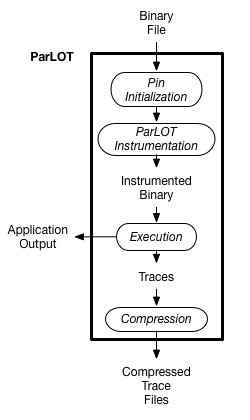
\includegraphics[width=2.2in]{parlot/overview3.png}
\caption{Overview of \parlot}
\label{overview}
\end{figure}


\subsection{Tracing Operation}
\label{subsec:traceOp}

\parlot uses the PIN API as its instrumentation mechanism to gather traces. In particular, it instructs \pin to instrument every thread launch and termination in the application as well as every function entry and exit. The thread-launch instrumentation code initializes the per-thread tracing variables and opens a file into which the trace data from that thread will be written. The thread-termination code finalizes any ongoing compression, flushes out any remaining entries, and closes the trace file. \parlot assigns every static function in each image (main program and all libraries) a unique unsigned 16-bit ID, which it records in a separate file together with the image and function name. This file allows the trace reader to map IDs back to function-name/image pairs.

For every function \emph{entry}, \parlot executes extra code that has access to the thread ID, function ID, and current stack-pointer (SP) value. Based on the SP value, it performs call-stack correction if necessary (see \S\ref{subsec:stack_cor}), adds the new function to a data structure it maintains that holds the call stack (which is separate from the application's runtime stack), and emits the function ID into the trace file via an incremental compression algorithm (see \S\ref{subsec:incr-compr}). All of this is done independently for each thread. Similarly, for every function \emph{exit}, \parlot also executes extra code that has access to the thread ID, function ID, and current SP value. Based on the SP value, it performs call-stack correction if necessary, removes the function from its call-stack data structure, and emits the reserved function ID of zero into the trace file to indicate an exit. As before, this is done via an incremental compression algorithm. We use zero for all exits rather than emitting the function ID and a bit to specify whether it is an entry or exit because using zeros results in more compressible output. This way, half of the values in the trace will be zero.





\subsection{Incremental Compression}
\label{subsec:incr-compr}

\parlot immediately compresses the traced information even before it is written to memory. It does, however, keep a sliding window (circular buffer) of the most recent uncompressed trace events, which is needed by the compressor. It compresses each function ID before the next function ID is known. The conventional approach would be to first record uncompressed function IDs in a buffer and later compress the whole buffer once it fills up. However, this makes the processing time very non-uniform. Whereas almost all function IDs can be recorded very quickly since they just have to be written to the buffer, processing a function ID that happens to fill the buffer takes a long time as it triggers the compression of the entire buffer. This results in sporadic blocking of threads during which time they make no progress towards executing the application code. Initial experiments revealed that such behavior can be detrimental when one thread is polling data from another thread that is currently blocked due to compression. For example, we observed a several order of magnitude increase in entry/exit events of an internal MPI library function when using block-based compression.

To remedy this situation, the compressor must operate incrementally, i.e., each piece of trace data must be compressed when it is generated, without buffering it first, to ensure that there is never a long-latency compression delay. Few existing compression algorithms have been implemented in such a manner because it is more difficult to code up and probably a little slower. Nevertheless, we were able to implement our algorithm (discussed next) in this way so that each trace event is compressed with similar latency.


\subsection{Compression Algorithm}
\label{subsec:compAlg}

We used the CRUSHER framework~\cite{mb-cluster15, mb-space16, mb-sc16, mb-dcc18} to automatically synthesize an effective and fast lossless compression algorithm for our traces. CRUSHER is based on a library of data transformations extracted from various compression algorithms. It combines these transformations in all possible ways to generate algorithm candidates, which it then evaluates on a set of training data. We gathered uncompressed traces from some of the Mantevo miniapps~\cite{mantevo} for this purpose. This evaluation revealed that a particular word-level Lempel-Ziv (LZ) transformation followed by a byte-level Zero-Elimination (ZE) transformation works well. In other words, \parlot 's trace entries, which are two-byte words, are first transformed using LZ. The output is interpreted as a sequence of bytes, which is transformed using ZE for further compression. The output of ZE is written to secondary storage.

LZ implements a variant of the LZ77 algorithm~\cite{LZ}. It uses a 4096-entry hash table to identify the most recent prior occurrence of the current value in the trace. Then it checks whether the three values immediately before that location match the three trace entries just before the current location. If they do not, the current trace entry is emitted and LZ advances to the next entry. If the three values match, LZ counts how many values following the current value match the values following that location. The length of the matching substring is emitted and LZ advances by that many values. Note that all of this is done incrementally. The history of previous trace entries available to LZ for finding matches is maintained in a 64k-entry circular buffer.

ZE emits a bitmap in which each bit represents one input byte. The bits indicate whether the corresponding bytes are zero or not. Following each eight-bit bitmap, ZE emits the non-zero bytes.

As mentioned above, we had to implement the two transformations incrementally to minimize the maximum latency. This required breaking them up into multiple pieces. Depending on the state the compressor is in when the next trace entry needs to be processed, the appropriate piece of code is executed and the state updated. If the LZ code produces an output, which it only does some of the time, then the appropriate piece of the ZE code is executed in a similar manner.


\subsection{PIN and Call-Stack Correction}
\label{subsec:stack_cor}

To be able to decode the trace, i.e., to correctly associate each exit with the function entry it belongs to, our trace reader maintains an identical call-stack data structure. Unfortunately, and as pointed out in the \pin documentation~\cite{pinurl}, it is not always possible to identify all function exits. For example, in optimized code, a function's instructions may be inlined and interleaved with the caller's instructions, making it sometimes infeasible for \pin to identify the exit. As a consequence, we have to ensure that \parlot works correctly even when \pin misses an exit. This is why the SP values are needed.

During tracing, \parlot not only records the function IDs in its call stack but also the associated SP values. This enables it to detect missing exits and to correct the call stack accordingly. Whenever a function is entered, it checks if there is at least one entry in the call stack and, if so, whether its SP value is higher than that of the current SP. If it is lower, we must have missed at least one exit since the runtime stack grows downwards (the SP value decreases with every function entry and increases with every exit). If a missing exit is detected in this manner, \parlot pops the top element from its call stack and emits a zero to indicate a function exit. It repeats this procedure until the stack is empty or its top entry has a sufficiently high SP value. The same call-stack correction technique is applied for every function exit whose SP value is inconsistent. Note that the SP values are only used for this purpose and are not included in the compressed trace.

The result is an internally consistent trace of function entry and exit events, meaning that parsing the trace will yield a correct call stack. This is essential so that the trace can be decoded properly. Moreover, it means that the trace includes exits that truly happened in the application but that were missed by \pin. Note, however, that our call-stack correction is a best-effort approach and may, in rare cases, temporarily not reflect what the application actually did. For example, this can happen for functions that do not create a frame on the runtime stack. When implementing \parlot on top of another DBI framework, call-stack correction may not be needed, resulting in even lower \parlot overhead.


\section{Evaluation}
\label{sec:evaluation}
\begin{figure}[t]
\begin{minipage}{.48\textwidth}
\centering
  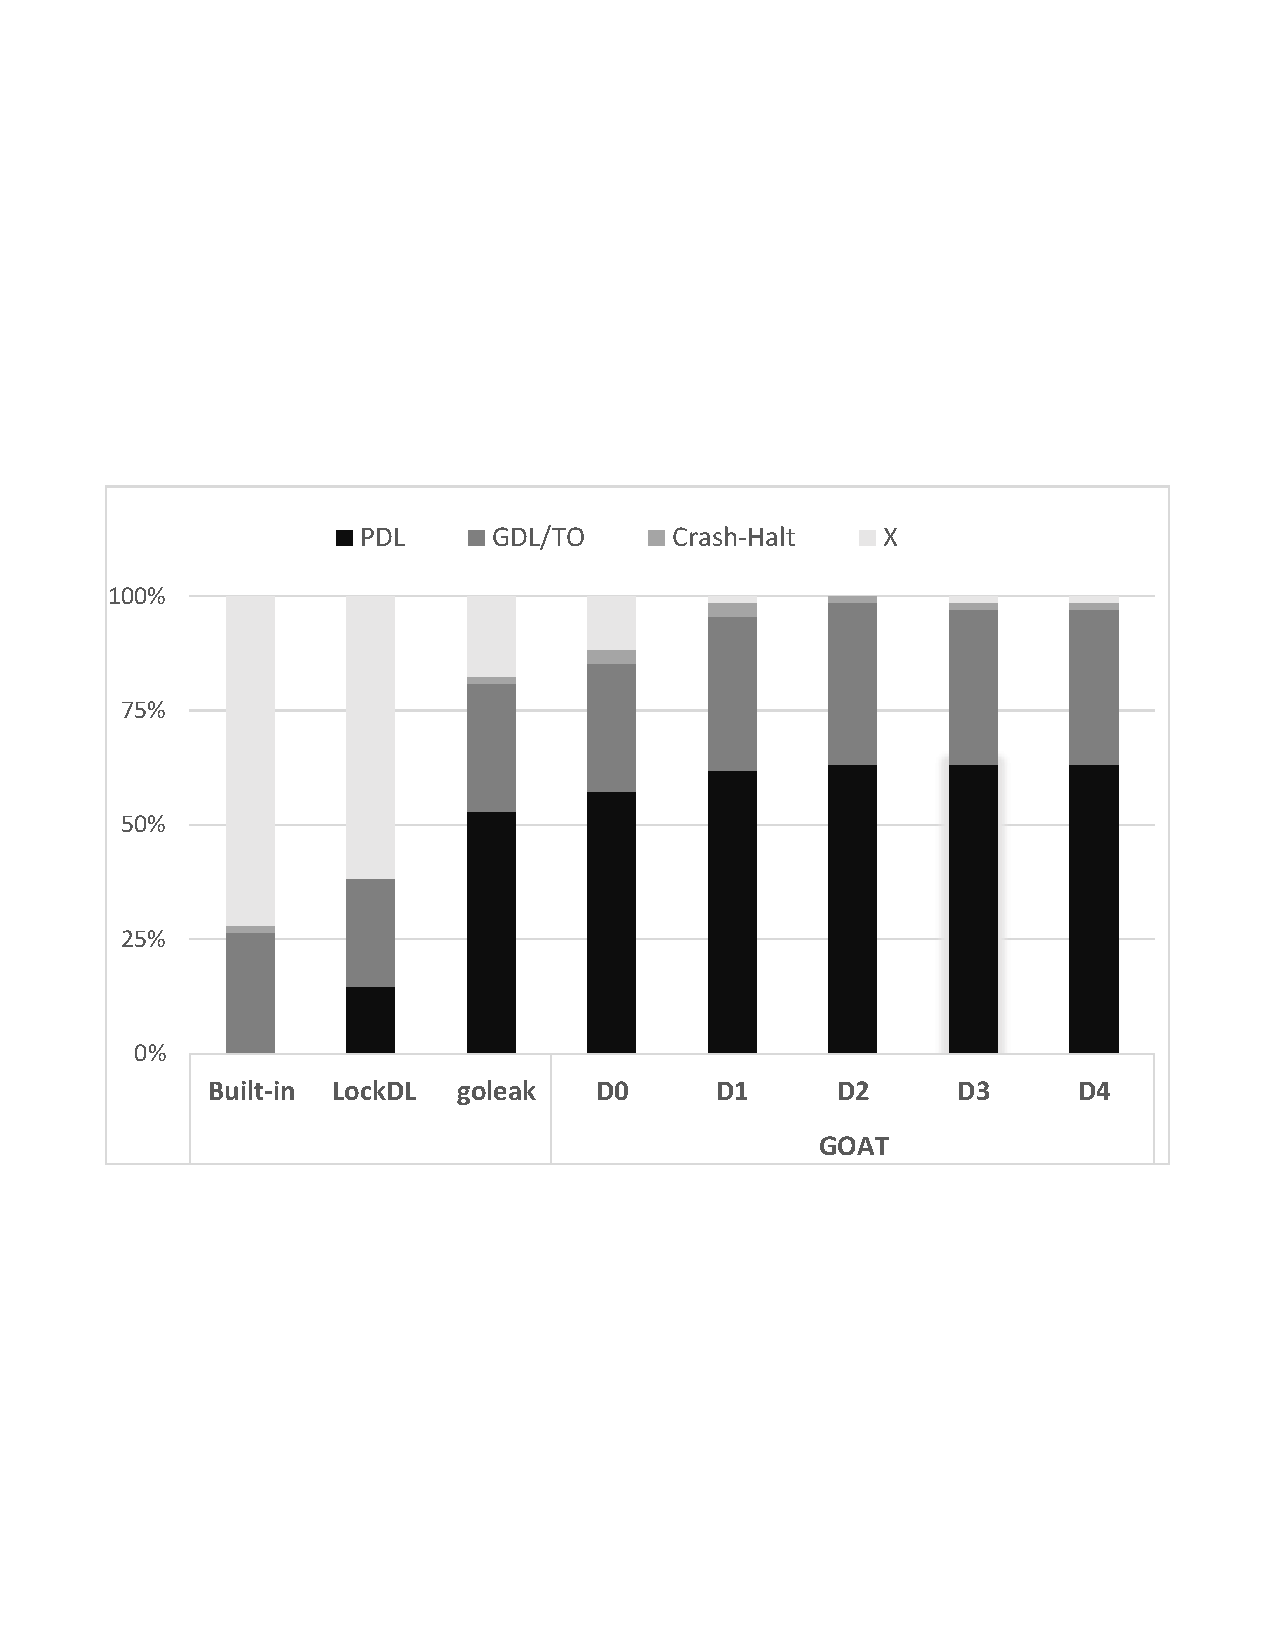
\includegraphics[width=.95\linewidth]{goat/figs/P4_detections.pdf}
  \caption{Histogram of detected bugs by each tool performed on 68 GoKer blocking bugs. PDL: partial deadlock, GDL/TO: global deadlock, Crash/Halt: causes the program to crash or halt during detection, X: nothing is detected }
  \label{fig:detection}
\end{minipage}
\begin{minipage}{.48\textwidth}
\centering
  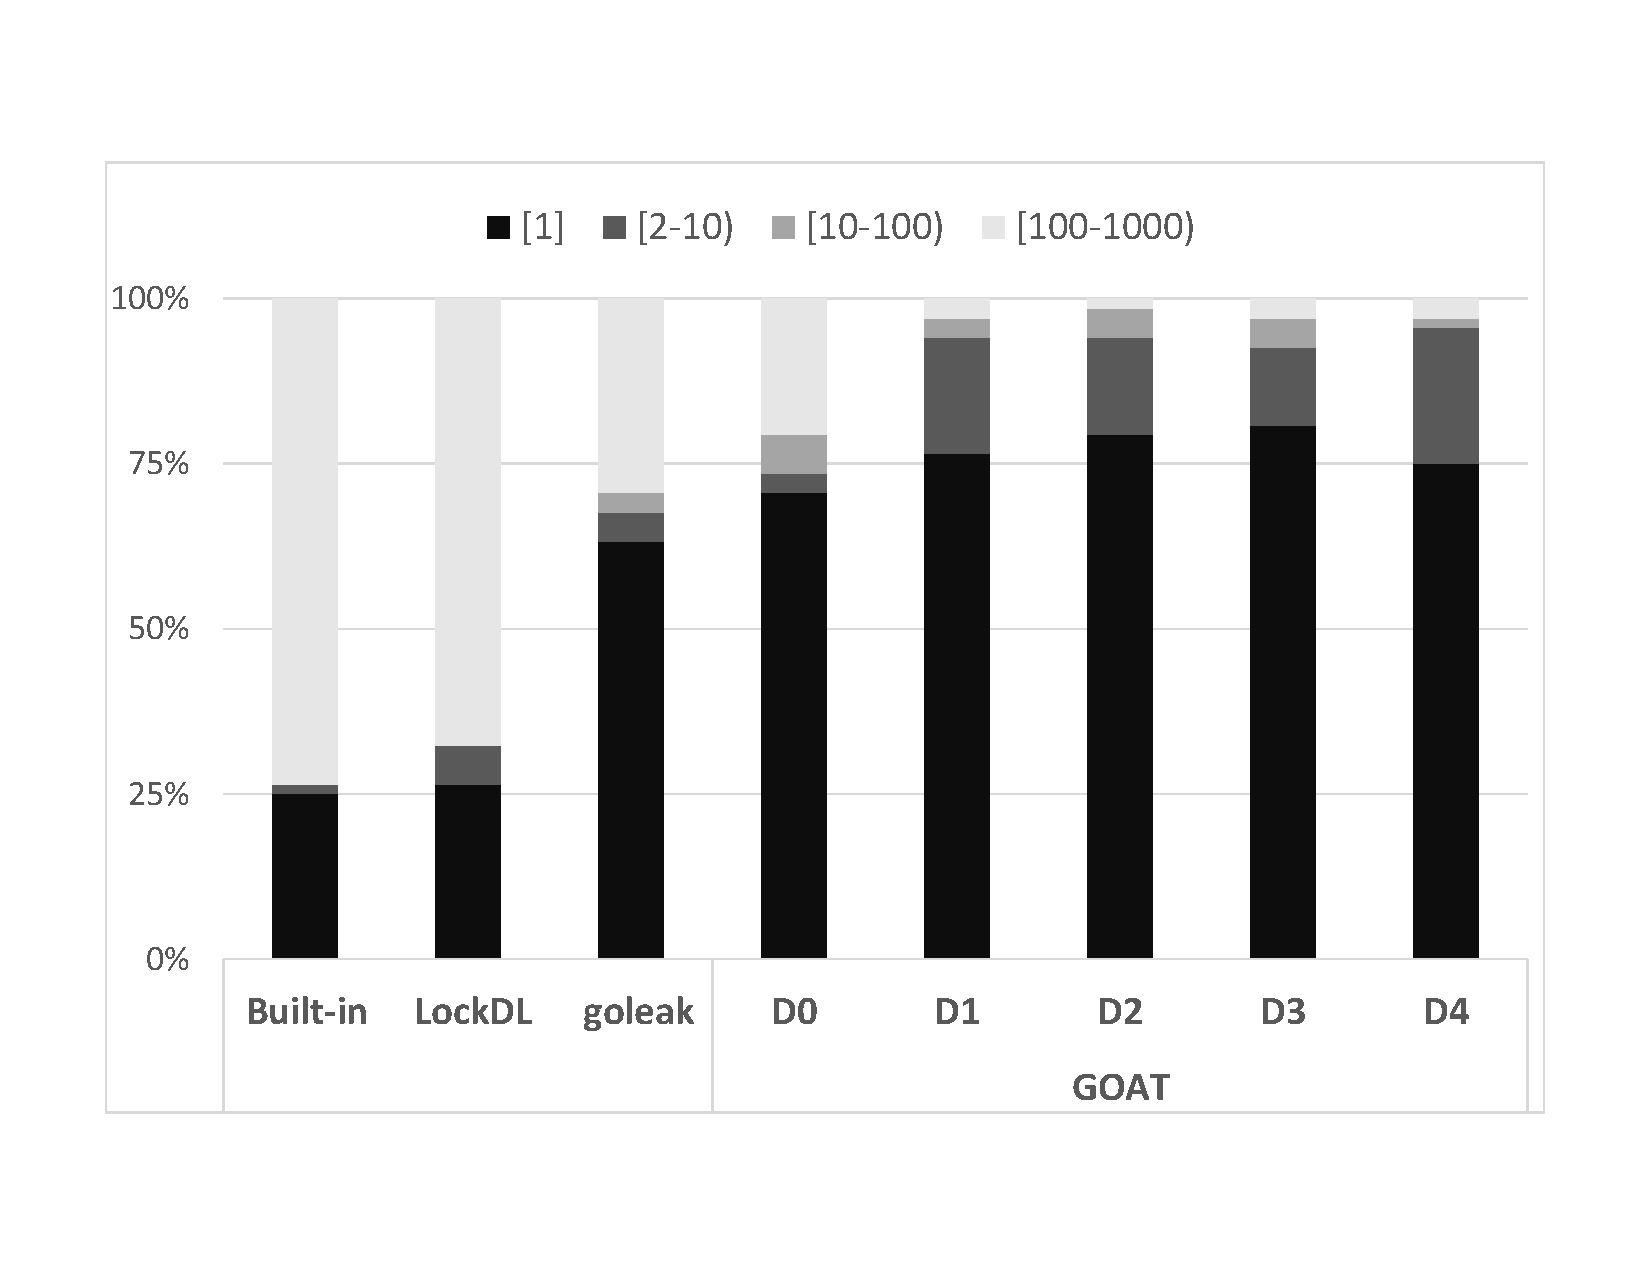
\includegraphics[width=.95\linewidth]{goat/figs/P4_runs.pdf}
  \caption{Histogram of required number of iterations by each tool to detect 68 GoKer blocking bugs}
  \label{fig:runs}
\end{minipage}
\end{figure}

\subsection{Deadlock Detection}
\label{sec:dl_evaluation}
We assess the ability of \goat and its variations in detecting bugs with minimum number of executions required to expose the bug.
%
We have compared \goat against three existing dynamic detectors:
\begin{itemize}
  \item \textit{Built-in} deadlock detector: It is an embeded mechanism in the standard Go runtime. The mechanism periodically makes sure that the queue of \textit{runnable} goroutines is never empty until the main goroutine terminates. If the queue is empty and main has not terminated yet (\ie main is blocked), it throws a runtime error.
  \item \textit{LockDL} \cite{lockdl}: This tool intercept with all mutex locks and unlocks of the target application to maintain a ``lock-set'' data structure. \textit{LockDL} issues warning during runtime when it finds a circular wait in the lock-set or double-locking the same lock. It has a timeout mechanism for application that traps into global deadlocks (30 seconds by default).
  \item \textit{goleak} \cite{goleak}: This leak detector from Uber checks the program stack at the end of the main goroutine's execution to find the application-level goroutines that remained in the stack (\ie leaked).
\end{itemize}

All experiments are performed on a server with two AMD Ryzen 5 3600 6-Core Processor (12 total cores with 2 threads per core and 6 cores per socket), 64 GB of RAM with generic Ubuntu 4.15.0 and Go version 1.15.6.
%
Table \ref{tab:comparison} shows the details of results obtained from executing each tool per bug 1000 times.
%
We show that the tool is unable to detect the bug after 1000 executions with \textbf{X (1000)}.
%

%
Figure \ref{fig:detection} and table \ref{tab:comparison} show that variations of \goat outperforms other detector by discovering the bug in 100\% of the GoKer blocking benchmark.
%
Figure \ref{fig:runs} and highlighted cells of table \ref{tab:comparison} show that the idea of injecting random delays around concurrency usage points in the program drastically reduces the required number of testing iterations until the bug occur.
%
D0 means \goat did not delay the program at any point and D4 means that the target program has been delayed up to four times around its CU points.
%
Figures \ref{fig:detection} and \ref{fig:runs} also state that the increase in the delay bound of \goat does not necessarily increase the chance of exposing the bug.
%
For example, the row of bug \texttt{serving\_2137} in table \ref{tab:comparison} show that only \goat D2 were able to detect the bug.


\begin{figure}[b]
\begin{minipage}{.48\textwidth}
\centering
  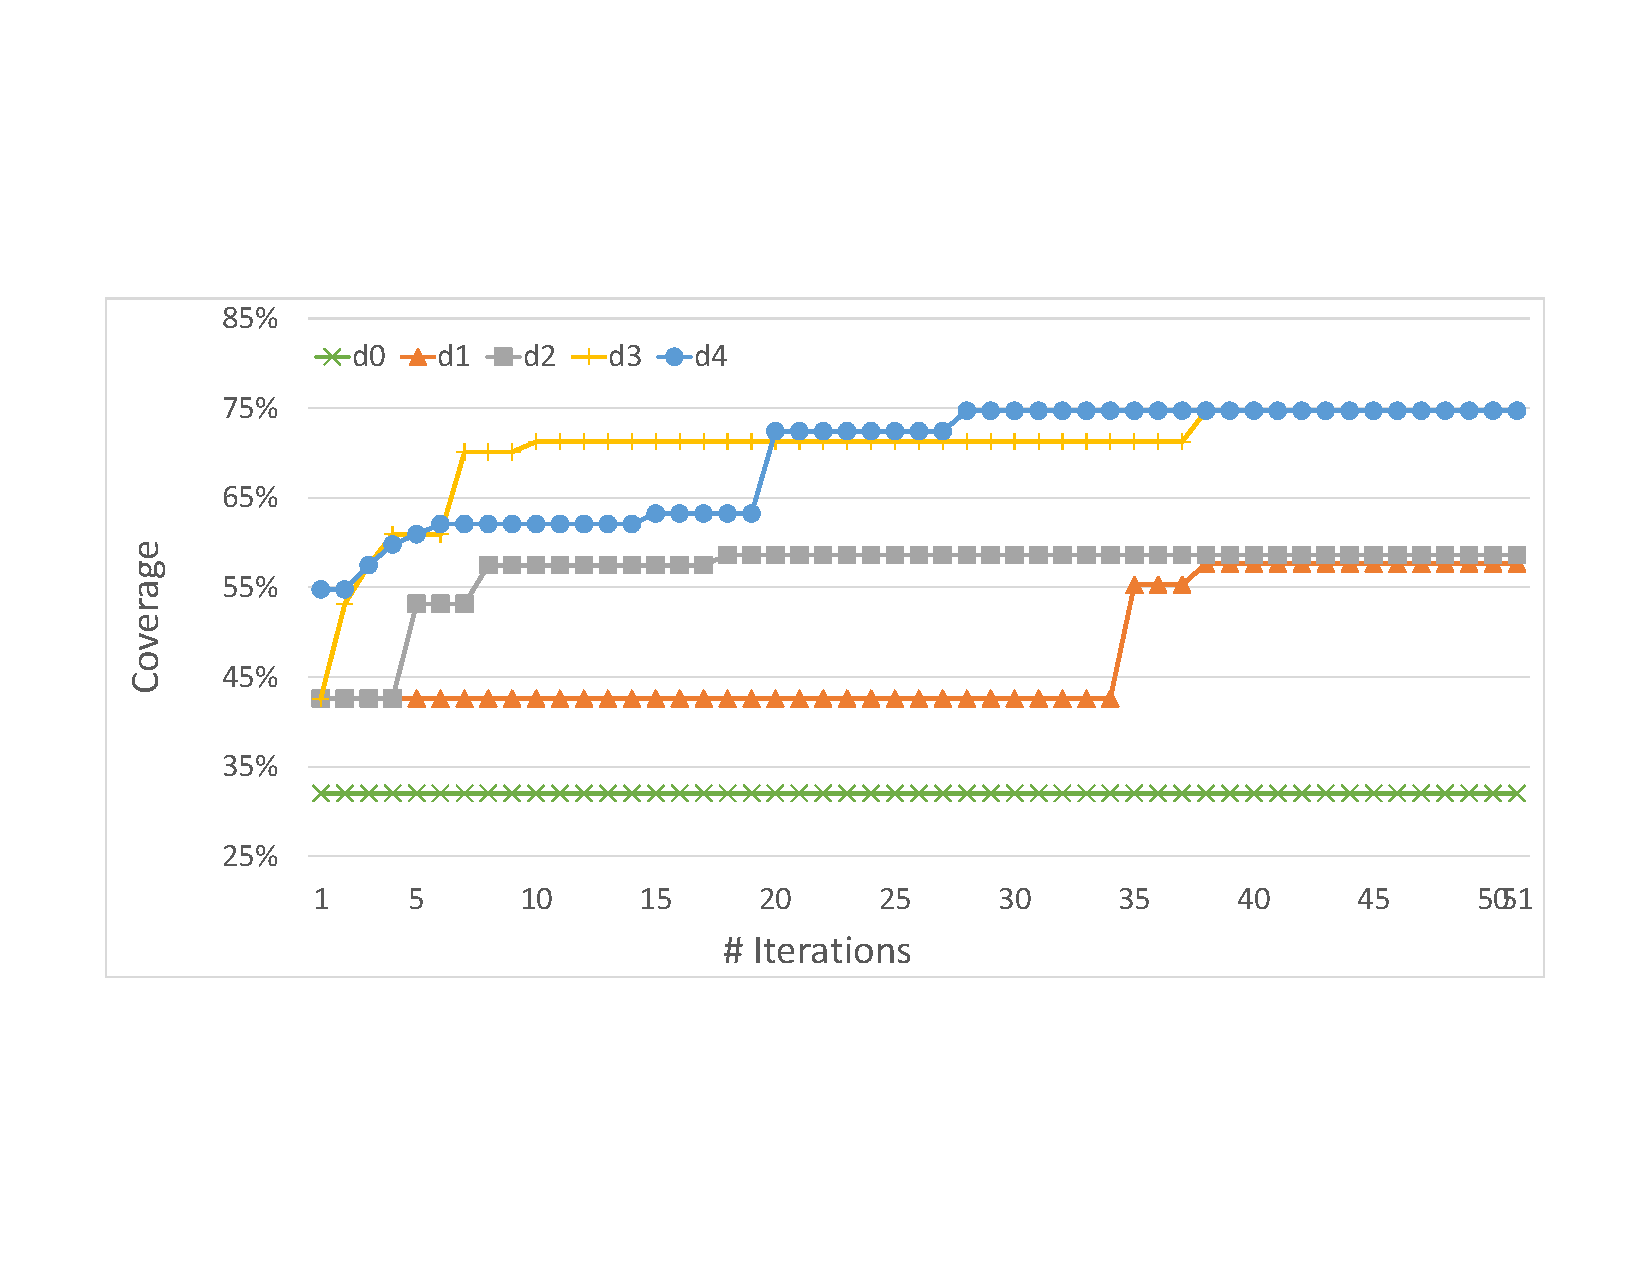
\includegraphics[width=.99\textwidth]{goat/figs/coverage_etcd7443.pdf}
  \caption{etcd7442 coverage}
  \label{fig:etcd_coverage}
\end{minipage}
\begin{minipage}{.48\textwidth}
\centering
  \includegraphics[width=.99\linewidth]{goat/figs/coverage_kubernetes11298.pdf}
  \caption{kuberenetes11298 coverage}
  \label{fig:kubernetes_coverage}
\end{minipage}
\end{figure}

\subsection{Coverage Analyis}
We picked two representative bug kernels \texttt{etcd7443} and \texttt{kubernetes11298} to evaluate the coverage idea on them as they
%
both have extensive use of channels, mutexes, conditional variables, nested selects within nested for loops and the buggy interleaving is proved to be rare to happen.
%
figures \ref{fig:etcd_coverage} and \ref{fig:kubernetes_coverage} show the gradual increase in coverage percentage during execution runs for different values of D.
%
Recall that D is the bound on the number of yields that we inject to the native execution of a given program to perturb the scheduler around concurrency usages.
%
These figures show that the increase of number of delays grows the rate of coverage percentage.
%
However, higher number of delays do not necessarily increase the coverage (D2 and D4 in figure \ref{fig:kubernetes_coverage}).
%
The drop in coverage for D1 in figure \ref{fig:kubernetes_coverage} is because of the new coverage requirements (\eg, a new goroutine is spawned and executing some concurrency primitives) that were encountered during testing execution.


%\section{GOAT: Coverage}
%\label{sec:coverage}
%
To demonstrate that testing has been thorough, \textit{coverage metrics} are defined to measure the progress of tests and specify testing termination condition.
%
Coverage metric for the set of testing executions $\mathcal{T}$ is a set of \textit{requirements} $\mathcal{R}$ that should get covered during testing iterations.
%
We say requirement $R_i$ is covered during testing iteration $t \in \mathcal{T}$ if we can correlate an \textit{action} during execution of $t$ to $R_i$.
%
For example, in \textit{statement coverage}, which is a widely-used metric in testing sequential software, $R$ is the set of source locations (file and line numbers) in the target program
%
$R_i$ is covered by test execution $t$ if the statement at location $R_i$ is executed in $t$.
%
The \textit{coverage percentage} of a test $\mathcal{T}$ is the ratio of the requirements covered by at least one execution over the number of all requirements ($|R|$).

As explained in Section \ref{sec:bg}, concurrent software testing frameworks perform testing iterations to explore the schedule-space and expose flaws.
%
Depending on the class of target bug, different coverage metrics are proposed and used for concurrent software testing.
%
\textit{Synchronization} coverage metrics such as \textit{blocking-blocked} \cite{edelstein2003contest}, \textit{blocked-pair-follows} \cite{trainin-followsCoverage-padtad09} and \textit{synchronization-pair} \cite{hong-syncTesting-issta12} defined requirements to cover during testing for exposing blocking bugs (\eg deadlocks).
%
%\textit{Memory access} coverage metrics such as PSet \cite{yu-pser-isca09} and def-use \cite{yang-defuse-issta98} focuses on data-access related bugs such as atomicity violation or data races.
%
For example, the synchronization coverage model in \cite{edelstein2003contest} defines \textit{blocking} and \textit{blocked} requirements per each synchronized block (\ie mutually exclusive section of the code that is protected by a lock).
%
The purpose of this requirement is to check if a test can report when there is a lock contention for two or more threads entering the synchronized block.
%
That is, a thread is either \textit{blocked} from entering the synchronization block or \textit{blocking} other threads from entering by holding the lock.
%

Proposed concurrency coverage metrics are mostly in the context of Java and C/Pthreads and are not directly applicable to languages like Go as Go has different concurrncy primitives and semantics.
%
Bron et. al,\cite{bron-appSyncCov-ppopp05} enumerates four major characteristics for coverage metrics to gain acceptance:
\begin{itemize}
  \item \textbf{Fixed model:} The metric should be well-understood by the developer or tester. A static model of requirements from target program should be constructed by instrumenting the source-code. The model should maintain covered requirements during testing executions.
  \item \textbf{Coverable and measurable requirements:} The absolute majority of reqiurements should be realistic enough to be \textit{coverable} during testing. For a few that are not coverable (due to program semantics) or not \textit{measurable} (because of technical limitations), the devloper should be aware of the reason.
  \item \textbf{Actions for uncovered requirements:} After testing terminates, every uncovered requirement should yield an action (\eg extending testing iterations or removing dead code from the program thus removing uncoverable requirements)
  \item \textbf{Coverage satisfaction:} Some action should be taken upon reaching a threshold of coverage percentage (e.g., testing phase termination when reaching 100\% statement coverage)
\end{itemize}

Defining a new coverage metric to satisfy above characteristics requires an accurate and proper mental model of target bugs.
%
Based on our observations from execution of Go applications and bug kernels on the behavior of concurrency primitives, we define a set of coverage requirements (summarized in Table \ref{tab:cov_req}):
%
\begin{itemize}
  \item \textbf{Req1 (Send/Recv):} \{\texttt{blocked}, \texttt{unblocking}, \texttt{NOP}\} -- Goroutine $G_1$ is either \textit{blocked} on a channel send (receive) if the receiver (sender) goroutine $G_2$ is not ready or \textit{unblocking} the waiting receiver (sender) goroutine $G_2$. A channel send or receive might also be neither blocked nor unblocking (NOP) for buffered channels.
  \item \textbf{Req2 (Select-Case):} \{\texttt{blocked}, \texttt{unblocking}, \texttt{NOP}\} $\times$ \{\texttt{case}$_i$\} -- cases of select statements are channel sends and recives (or default case for non-blocking selects). For all select statements that has no default case, we obtain the cases of each select statement at runtime and maintain an instance of Req1 per case.
  \item \textbf{Req3 (Lock):} \{\texttt{blocked}, \texttt{blocking}\} -- Goroutine $G_i$ is either \textit{blocked} when locking a mutex because another goroutine has locked the mutex or \textit{blocking} other goroutines from acquiring the mutex lock.
  \item \textbf{Req4 (Unblocking):} \{\texttt{unblocking}, \texttt{NOP}\} -- The goroutine that is performing channel close, mutex unlock, conditional variable signal and broadcast, waitGroup done and non-blocking select case (send or receive) has two kinds of behavior. They either \textit{unblock} one or more waiting goroutines or has no effect (NOP).
  \item \textbf{Req5-Go:} \{\texttt{NOP}\} -- We emit a NOP action for each goroutine creation to indicate that it is covered during testing.
\end{itemize}


These requirements are effective because with the help of \goat infrastructure, they satisfy the characteristics of an ``acceptable'' coverage metric:
\begin{itemize}
  \item A \textit{fixed concurrency model} from target application is statically obtained by identifying CU points.
  \item We can measure whether the requirement has been covered by analyzing the test ECT. By maintaining a global data structure during execution of all $t \in \mathcal{T}$, we can evaluate the coverability of proposed requirements
  \item Every uncovered requirement report something meaningful. For example, if a send is always performing as \textit{unblocking} and never as \textit{blocked}, which means that receiver of this send always performs receive before sender reaches its send statement. In other words, the receive action \textit{always happen-before} send action. Perhaps this pattern of communication is part of the program semantic and matches developer's expectations (e.g., a set of goroutines are listening on a channel to perform non-frequent requests). Otherwise, it reflects a bug or flaw in the program design.
  \item Since \goat is able to detect occured blocking bugs and also maintain a global coverage model during testing iterations, testing phase can terminate either by detection of a bug or reaching a coverage percentage threshold.
\end{itemize}

Table \ref{tab:moby_cov_table} shows a representation of covered requirements after a successful run (run \#1) and a leaky execution (run \#2) of the program in listing \ref{listing:moby28462.minipage}.
%
The highlighted cells of the table are the requirements that were not covered in the successful run \#1 but covered in run \#2 in which the bug has revealed.
%



\begin{table}[]
\centering
\caption{Coverge requirements defined for concurrent Go}
\scalebox{0.9}{
\begin{tabular}{|
>{\columncolor[HTML]{FFFFFF}}l |
>{\columncolor[HTML]{FFFFFF}}l |
>{\columncolor[HTML]{FFFFFF}}c |
>{\columncolor[HTML]{FFFFFF}}c |
>{\columncolor[HTML]{FFFFFF}}c |
>{\columncolor[HTML]{FFFFFF}}c |}
\hline
\multicolumn{1}{|c|}{\cellcolor[HTML]{FFFFFF}} & \multicolumn{1}{c|}{\cellcolor[HTML]{FFFFFF}} & \multicolumn{4}{c|}{\cellcolor[HTML]{FFFFFF}Coverage Requirement Types} \\ \cline{3-6}
\multicolumn{1}{|c|}{\multirow{-2}{*}{\cellcolor[HTML]{FFFFFF}\begin{tabular}[c]{@{}c@{}}Coverage\\ Requirements\end{tabular}}} & \multicolumn{1}{c|}{\multirow{-2}{*}{\cellcolor[HTML]{FFFFFF}\begin{tabular}[c]{@{}c@{}}Concurrent\\ Action\end{tabular}}} & Blocked & Unblocking & Blocking & NOP \\ \hline
\cellcolor[HTML]{FFFFFF} & SEND & * & * &  & * \\ \cline{2-6}
\multirow{-2}{*}{\cellcolor[HTML]{FFFFFF}Req. 1: Send/Recv} & RECV & * & * &  & * \\ \hline
\cellcolor[HTML]{FFFFFF} & CASE$_i$ (SEND) & * & * &  & * \\ \cline{2-6}
\multirow{-2}{*}{\cellcolor[HTML]{FFFFFF}Req. 2: Select-Case} & CASE$_i$ (RECV) & * & * &  & * \\ \hline
Req. 3: Lock & LOCK & * &  & * &  \\ \hline
\cellcolor[HTML]{FFFFFF} & CLOSE &  & * &  & * \\ \cline{2-6}
\cellcolor[HTML]{FFFFFF} & UNLOCK &  & * &  & * \\ \cline{2-6}
\cellcolor[HTML]{FFFFFF} & SIGNAL &  & * &  & * \\ \cline{2-6}
\cellcolor[HTML]{FFFFFF} & BRDCST &  & * &  & * \\ \cline{2-6}
\multirow{-5}{*}{\cellcolor[HTML]{FFFFFF}Req. 4: Unblocking} & NB-SELECT &  & * &  & * \\ \hline
Req. 5: Go & Go &  &  &  & * \\ \hline
\end{tabular}

}
\label{tab:cov_req}
\end{table}



%\textbf{Req5-Wait:} \{\texttt{blocked},\texttt{non-blocking}\} -- the goroutine that performs a conditional variable or waitGroup Wait is either blocked waiting for a wake-up signal from other goroutines or is non-blocking when

\begin{figure}
\centering
  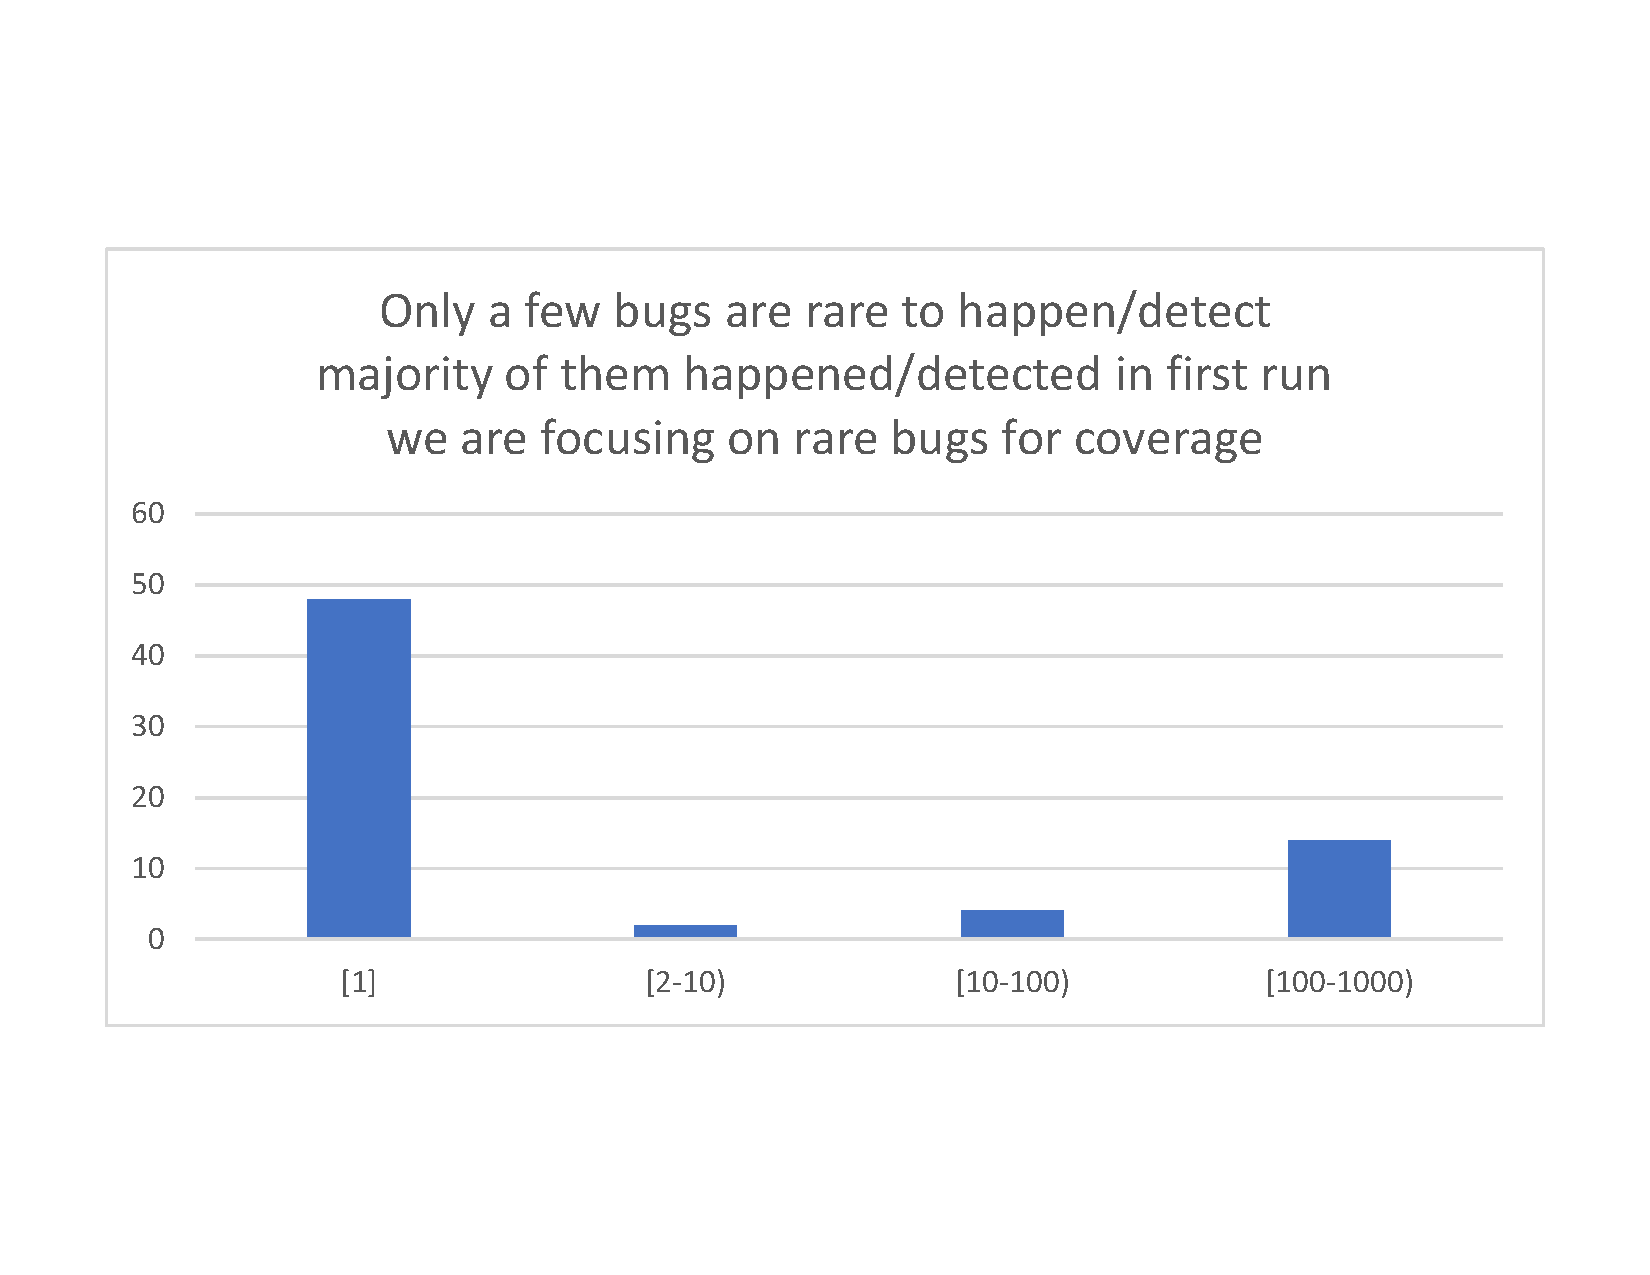
\includegraphics[width=.95\linewidth]{figs/coverage_motivation_tentative.pdf}
  \caption{focusing on rare bugs}
  \label{fig:rare_bugs}
\end{figure}



\subsection{Implementation}
Through a replay (\ie parsing the sequence) of ECT, a mapping between dynamic concurrent events and statically obtained CU points is emited by matching their respective call-stack and CU source location.
%
Through a BFS traversal of the goroutine tree, we add a \textit{coverage vector} to each goroutine node from the emitted mapping. Each element of the coverage vector is the respective covered value of requirement $R_i$ for the current goroutine node.
%
During executions of tests $t \in \mathcal{T}$, we maintain and update a global goroutine tree after each $t$.
%
It is crucial to maintain a global goroutine tree to measure the progress of coverage percentage over tests in $\mathcal{T}$.
%
Two goroutines $G_m$ and $G_n$ in the tests $t_i$ and $t_j$ are \textit{equivalent} (\ie falls into identical node in the global goroutine tree) if their parents are equivalent and their creation source location (CU of kind \texttt{go}) are identical:
\begin{equation}
  G_m \equiv G_n   \text{if}
  \begin{cases}
    \text{parent}(G_m) \equiv \text{parent}(G_n)  \wedge \\
    \text{CU(}G_m\text{).file} = \text{CU(}G_n\text{).file}  \wedge\\
    \text{CU(}G_m\text{).line} = \text{CU(}G_n\text{).line} \\
  \end{cases}
\end{equation}





\subsection{Evaluation}
We picked two representative bug kernels \texttt{etcd7443} and \texttt{kubernetes11298} to evaluate the coverage idea on them as they
%
They both have extensive use of channels, mutexes, conditional variables, nested selects within nested for loops and the buggy interleaving is proved to be rare to happen.
%
figures \ref{etcd_coverage} and \ref{fig:kubernetes_coverage} show the gradual increase in coverage percentage during execution runs for different values of D.
%
Recall that D is the bound on the number of yields that we inject to the native execution of a given program to perturb the scheduler around concurrency usages.
%
These figures show that
%


\begin{figure}
\centering
  \includegraphics[width=.95\linewidth]{figs/coverage_kubernetes11298.pdf}
  \caption{kuberenetes11298 coverage}
  \label{fig:kubernetes_coverage}
\end{figure}



\section{Related Work}
\label{sec:related}
Three major recent studies
have emphasized the need for better debugging tools
{\em and} the need to build a community that can share debugging
methods and infrastructure: the DOE report mentioned
earlier \cite{hpcdoe},
an NSF workshop~\cite{Cohen:2018:IRC:3297279}, and an ASCR report on
extreme heterogeneity~\cite{ascr-report-extreme-heterogeneity}.
%
Our key contribution in this paper is a fresh approach to debugging
that (1)~incorporates methods to debug across the API-stack
by resorting to binary tracing and thereby being able to ``dial into''
MPI bugs and/or OpenMP bugs (as shown in the ILCS case study), (2)~makes
initial triage of debugging methods possible via function-call traces,
and (3)~enables the verification community to cohere around DiffTrace
by allowing other tools to extend our toolchain (they can tap into it at various places).


Many HPC debugging efforts have emphasized
the need to highlight dissimilarities and
incorporate progress measures on loops. We now
summarize a few of them.
%
AutomaDeD~\cite{automaded-GBron}\cite{automaded-laguna}
captures the application's control flow
via Semi Markov Models and detects outlier executions.
%
PRODOMETER~\cite{prodometer} detects loops in
AutomaDeD models and introduces the
notion of {\em least progressed tasks} by analyzing {\em progress dependency graphs}.
%
DiffTrace's DiffNLR method does not (yet) incorporate progress measures; it only
computes changes in loop {\em structure}.
%
Prodometer's methods are ripe for symbiotic incorporation into DiffTrace.
%
We also plan to incorporate {\em happens-before} computation as a progress measure using FCA-based algorithms by Garg et al.~\cite{latticeForDistConst,garg_2015}.
%
FCA-based approaches have been widely used in data mining~\cite{cldm},
machine learning~\cite{clml}, and information retrieval \cite{ignatov17}.


In terms of computing differences with previous executions,
we draw inspirations from
Zeller's delta-debugging~\cite{DBLP:conf/esec/Zeller99}
and De Rose et al.'s relative debugging~\cite{relative-debugging}.
%
The power of equivalence classes for outlier detection is
researched in STAT~\cite{stat}, which
merges stack traces from processes into a prefix tree,
looking for equivalence-class outliers.
%
STAT uses the StackWalker API from Dyninst~\cite{dyninst} to gather stack traces
and efficiently handles scaling issues
through tree-based overlay networks such as MRnet~\cite{mrnet}.
%
D4~\cite{liu-18} detects concurrency bugs by statically analyzing source-code
changes, and DMTracker~\cite{dmtracker} detects anomalies in data movement.
%
The communication patterns of HPC applications can be automatically characterized by
diffing the communication matrix with common patterns~\cite{roth-15} or by
detecting repetitive patterns~\cite{preissl-08}.
%
ScalaTrace~\cite{scalatrace} captures and compresses communication traces for later replay. 
%
Synoptic~\cite{beschastnikh-synoptic} is applied to distributed
system logs to find bugs.
%
%Ravel~\cite{ravel} systematically visualizes large-scale application communications~\cite{charmVis}. 

%
%
%\subsection{OTHERS}
%\hl{in case of lack of material}
%\begin{itemize}
%\item Trace File Comparison with a hierarchical Sequence Alignment algorithm \cite{weber-seqAlign}
%\item structural clustering : matthias weber \cite{weberStructural}
%\item building a better backtrace: techniques for postmortem program analysis - ben liblit \cite{liblit02}
%\item automatically charecterizing large scale program behavior - timothy sherwood \cite{sherwood02}
%\item Score-P \cite{scorep}
%\item TAU \cite{tau}
%\item ScalaTrace: Scalable compression and replay of communication traces for HPC  \cite{scalatrace}
%\end{itemize}






%
%\subsection{STAT}
%
%Parallel debugger STAT\cite{stat}
%\begin{itemize}
%\item STAT gathers stack traces from all processes
%\item Merge them into prefix tree
%\item Groups processes that exhibit similar behavior into equivalent classes
%\item A single representative of each equivalence can then be examined with a full-featured debugger like TotalView or DDT
%\end{itemize}
%
%What STAT does not have?
%
%\begin{itemize}
%\item FP debugging
%\item Portability (too many dependencies)
%\item Domain-specific
%\item Loop structures and detection
%\end{itemize}





\section{Summary \& Future Work}
\label{sec:summary}
We presented \goat, an analysis and testing framework for concurrent Go applications to assist concurrency debugging of real-world applications.
%
\goat combines static and dynamic methods to model and explore application execution.
%
The scheduler behavior is pertubed with automatically injected random delays to accelerate the exposure of bug, if any.
%
By dynamic measurment of a set of coverage requirements, we quantify the quality of schedule-space exploration of \goat.
%
\goat detects all 68 blocking bugs of GoKer benchmark which are the bug kernels of top nine open-soruce projects written in Go.
%
The schedule perturbation showed effectiveness in accelerating the bug exposure.
%
Proposed coverage requirements accurately reflect the dynamic behavior of program executions and testing iterations.

Engineering of \goat is flexible and extensible to more advanced components.
%
For example, current minimal \goat engine can be extended to take the full control over the Go scheduler and ``guide'' testing towards untested interleaving.
%
We are dockerizing \goat for easy and public use.
%
We want to test on real-world programs.
%
The data that ECT includes is rich enough for training accurate models and apply machine learning methods to learn and predict bug patterns.



\bibliographystyle{IEEEtran}
\bibliography{bibs}


\end{document}
